%%%%%%%%%%%%%%%Conjectures regarding values of Riemann zeta function at Gram points%%%%%%%%%%%%%%%%%%%%%%%%%%%%%%%%%%%%%%%%%%%%%%%%%%%%%%%%%%%%%
%

\documentclass[twoside]{article}
\usepackage{graphicx}
\usepackage{amsmath,amsthm,amssymb,verbatim}
\usepackage{fancyhdr}
\pagestyle{fancy}
\usepackage{url}

\def\blfootnote{\xdef\@thefnmark{}\@footnotetext} 
\long\def\symbolfootnote[#1]#2{\begingroup%
\def\thefootnote{\fnsymbol{footnote}}\footnote[#1]{#2}\endgroup} 

\newtheorem{mydef}{Conjecture}

\setcounter{page}{1}
\begin{document}

\date{}
\lhead[]{}
\chead[]{}
\rhead[]{}

\title{\bf{Good to Bad Gram Point Ratio For Riemann Zeta Function}}
%

\author{O. Shanker 
 \thanks{Mountain View, CA 94041, U. S. A. Email: oshanker@gmail.com
 }
}

\maketitle
\thispagestyle{fancy}

\begin{abstract}
We consider the asymptotic value of the ratio of good to bad Gram points for the Riemann zeta function.
We relate this to a conjecture of Odlyzko about the locations of the zeros of the Riemann zeta function.
The conjecture is based on the GUE hypothesis, and the additional assumption that a Gram interval does not differ from any other interval of that length.
If the conjecture is correct, we show that the ratio of good to bad Gram points should be $1$. 
We study the empirical evidence for the relationship. The study leads us to the formulation of two 
symmetry related conjectures about the location of the zeros.
\end{abstract}



%\clearpage
\chead[\underline{O. Shanker}]{\underline{Good to Bad Gram Point Ratio For Riemann Zeta Function}}


\section{Introduction}
The Riemann Hypothesis is one of the seven millennium prize problems posed by the Clay Mathematical Institute in 2000~\cite{Sarnak 2005}. The earliest detailed evaluations of the roots of the Riemann zeta function were carried out in 1903 by Gram~\cite{Gram 1903}.
In evaluating the zeros he made use of the values of the Riemann zeta function at special (very regularly placed) points which are called "Gram points".
He observed that in his calculations the roots of the Riemann zeta function alternated with the Gram points. He also observed that the
value of the real part of the Riemann zeta function was positive at the Gram points. Such points are today called good Gram points. Thus, we may say that since the early 
twentieth century we have been observing that the majority of Gram points are good Gram points. In this work we study empirically the ratio of good to bad Gram points, and relate it to a conjecture of Odlyzko~\cite{Odlyzko 1992}. The conjecture is based on the GUE hypothesis, and the additional assumption that a Gram interval does not differ from any other interval of that length.
If the conjecture is correct, we show that the ratio of good to bad Gram points should be $1$. We also formulate two symmetry related conjectures about the location of the zeros.

The paper is organized as follows.
Section~\ref{sec2} establishes the required notation for the 
Riemann Zeta Function. 
Section~\ref{sec3} describes the Gram points. 
Section~\ref{sec4} describes the Gram blocks. 
In Section~\ref{sec5} we study empirically the ratio of good to bad Gram points, and relate it to a conjecture of Odlyzko. 
In Section~\ref{sec6} we study the ratio of $Type~II/Type~I$ Gram blocks.. 
Section~\ref{sec7} presents two new conjectures. 
Section~\ref{conclusions} gives a brief summary of the results. 

\section{\label{sec2}The Notation for the Riemann zeta function }

In this section we  establish the required notation for the 
Riemann Zeta Function. 
The Riemann Zeta function is defined for $\mathrm{Re} (s) > 1$ by
\begin{equation}
\zeta ( s ) \, = \, \sum^{\infty}_{n = 1} \; n^{-s} \, = \, \prod_{p \in primes} \;
\left( 1 - p^{-s} \right)^{-1}.
\label{eqRie}
\end{equation}

Eq.~(\ref{eqRie})  converges for $\mathrm{Re} (s) > 1$.  
 $\zeta ( s )$ has a  continuation
to the complex plane and satisfies a functional equation \cite{Riemann(1858),Riemann 1892, Titchmarsh 1986,Edwards(1974)}
\begin{equation}  
\xi(s):= \pi^{-s/2} \, \Gamma (s/2) \, \zeta ( s ) \, = \, \xi ( 1 - s );
\label{eq:func}
\end{equation}
$\xi(s)$ is entire except for simple poles at $s = 0$ and $1$. Riemann
multiplied the definition by $s(s-1)$ to remove the poles. We
write the zeroes of $\xi(s)$ as $1/2 + i \gamma$. The Riemann Hypothesis  
asserts that $\gamma$ is real for the non-trivial zeroes.
We order the $\gamma$s in increasing order, with 
\begin{equation}
\ldots \ldots \gamma_{-1} \, < \, 0 \, < \, 
\gamma_1 \, \leq \, \gamma_2 \ldots. 
\end{equation}
Then $\gamma_j \, = \, - \gamma_{-j}$ for $j = 1, 2, \ldots,$ 
and    $\gamma_1$, $\gamma_2$, $\ldots$  are roughly
$14.1347$, $21.0220$, $\ldots$.


Asymptotically, for the Riemann zeta function the mean number of 
zeros with height less than $\gamma$ (the smoothed Riemann zeta staircase)
is~\cite{Edwards(1974)}
\begin{equation}  
<\mathcal{N_R} (\gamma)> = (\gamma/2\pi)(ln(\gamma/2\pi)-1)-\frac{7}{8}.
\label{eq:Rnumber}
\end{equation}
Thus, the mean spacing of the zeros at height $\gamma$ is 
$2\pi(\ln (\gamma/2\pi))^{-1}$. 

The study of the zeroes of the Riemann zeta function and Generalized 
Zeta functions is of interest to mathematicians and physicists. Mathematicians 
study the spacings because of its applications to analytic number theory, 
while physicists study it because of its  relation 
to the theory of the spectra of random matrix theories (RMT) 
and the spectra of classically chaotic quantum systems. 
Many remarkable properties of the Riemann zeta function keep turning up in the literature~\cite{os6,Matiyasevich}.


The next section discusses the Gram Points.

\section{\label{sec3}Gram Points}

In this section we discuss the details of the numerical work. 
The numerical analysis takes advantage of the functional 
equation Eq.~(\ref{eq:func}).
One defines
\begin{equation}
\theta(t) = arg (\pi^{?it/2} \Gamma(\frac{1}{4} + \frac{it}{2})), 
\label{eq:theta}
\end{equation}
where the argument is defined by continuous variation of $t$ starting with the value $0$ at $t = 0$.
For large $t$ $\theta$ has the asymptotic expansion
\begin{equation}
\theta(t) = \frac{t}{2}\ln (\frac{t}{2\pi}) - \frac{t}{2} - \frac{\pi}{8} + \frac{1}{48t} - \frac{1}{5760t^3}. 
\label{eq:thetaAsymptotic}
\end{equation}
A consequence of the zeta functional equation is that the function 
$Z(t)=exp(i\theta(t))\zeta(1/2 +it)$,
known as the Riemann-Siegel Z-function, is real valued for real $t$. 
Moreover we have $|Z(t)| = |\zeta(1/2+it)|$. Thus the zeros of $Z(t)$ are the imaginary part of the zeros 
of $\zeta(s)$ which lie on the critical line. We are led to finding the change of sign 
of a real valued function 
to find zeros on the critical line. This is a very convenient property in the numerical verification 
of the Riemann Hypothesis.
Another very helpful property is that many of the zeros are separated by the
"Gram points".  When $t \ge 7$, the $\theta$ function Eq.(\ref{eq:theta}) is monotonic increasing. 
For $n \ge 1$, the $n-th$ Gram point $g_n$ is defined as the unique solution $> 7$ to
$\theta (g_n) = n\pi$.
The Gram points are as dense as the zeros of $\zeta(s)$ but are much more regularly distributed.
Their locations can be found without any evaluations of the Riemann-Siegal series Eq.(\ref{eq:RS}).
Gram's law is the empirical observation that $Z(t)$ usually changes its sign in each Gram interval 
$G_n = [g_n,g_{n+1})$. 
This law fails infinitely often, but it is true in a large proportion of cases.
The average value of $Z(g_n)$ is $2$ for even $n$ and $-2$ for odd $n$~\cite{Titchmarsh 1986},
and hence $Z(g_n)$ undergoes an infinite number of sign changes.


The Riemann-Siegel Z-function is evaluated using the Riemann-Siegal series
\begin{equation}
Z(t) = 2\sum^{m}_{n=1}\frac{\cos(\theta(t) - t \ln (n))}{\sqrt{n}} + R(t), 
\label{eq:RS}
\end{equation}
where $m$ is the integer part of $\sqrt{t/(2\pi)}$, and $R(t)$ is a small remainder
term which can be evaluated to the desired level of accuracy. The most important 
source for loss of accuracy at large heights is the cancellation between
large numbers that occur in the arguments of the $\cos$ terms in Eq.~(\ref{eq:RS}). We 
use a high precision module to evaluate the arguments. The rest of the calculation
is done using regular double precision accuracy. See ~\cite{hiary,gourdon,Odlyzko(1989)} for methods to efficiently evaluate the zeta function at large t.

In the next section we present the theory of Gram blocks.

\section{\label{sec4}Gram Blocks}


In this section we present the different types of Gram blocks. We will follow the notation of   Odlyzko~\cite{Odlyzko 1992}. A Gram point $g_n$ is called good if $(-1)^nZ(g_n) > 0$, and bad otherwise. A Gram block is an interval $[g_n, g_{n+k})$ such that $g_n$  and $g_{n+k}$ are good Gram points 
and $g_{n+1}, . . ., g_{n+k-1}$ are bad Gram points. A Gram block is denoted by the notation $a_1a_2 . . . a_k$ where k is called the length of the Gram block, and $a_i$ denote the number of roots of Z(t) in the Gram interval $[g_{n+i-1}, g_{n+i})$. So far, no Gram interval has been found with more than 5 zeros, thus the notation is unambiguous. $a_1$ and $a_k$ must be even while  $a_2$ to $a_{k-1}$ are odd.

A Gram block of length k which contains exactly k roots of Z[t) is called regular. The first and last Gram intervals of a regular Gram block must contain an even number of roots (0 or 2 roots). The internal Gram intervals must all contain an odd number of roots (all of them must contain one root if the end intervals contain 2 and 0 roots. If the end intervals both contain no roots, then one of the internal intervals must contain 3 roots.) 
Thus, regular Gram blocks must have a pattern of one of the following three forms:
$21 . . . 10, 01 . . . 12, 01 . . . 131 . . . 10$
where the notation $1 . . . 1$ refers to any string of consecutive 1s, including the zero length string. Odlyzko~\cite{Odlyzko 1992} denotes these three types of regular Gram Blocks as Type I, Type II and Type III respectively.  

In the next section we study the ratio of good to bad Gram points, and relate it to Odlyzko's conjecture.

\section{\label{sec5}Good to Bad Gram point ratio}

\begin{table}
\centering \(\begin{array}{llllll}
\hline
Source &m = 0&m = 1&m = 2&m = 3&size\\
\hline
t = 10^{12}&0.148797&0.704395&0.144823&0.001987&1000000\\
t = 10^{15}&0.1536533&0.6946820&0.1496761&0.0019886&10000000\\
t = 10^{28}&0.1619184&0.6781499&0.1579456&0.0019855&10000000\\
 GUE&0.170222&0.661430&0.166490&0.001860&\\
\hline
\end{array}\)
\caption{Counts of Gram intervals that contain $m$ zeros, and the GUE prediction.} \label{tab:intervalzeros}
\end{table}

\begin{table}
\centering \(\begin{array}{ccccccc}
\hline
Source &p_g&p_b& p_g/p_b&p_{even|bad} &p_{even|good}&\frac{p_{even|bad}}{p_{even|good}}\\
\hline
t = 10^{12}&0.7962&0.2038&3.9&0.7204&0.1844&3.9\\
t = 10^{15}&0.7792&0.2208&3.5&0.6868&0.1946&3.5\\
t = 10^{28}&0.7374&0.2626&2.8&0.6090&0.2169&2.8\\
\hline
\end{array}\)
\caption{Test from  Equation~\ref{eqGoodRelation} that the zero counts distribution in a Gram interval is not independent of Gram type.} \label{tab:pevenpred}
\end{table}

In this section we consider the distribution of Gram intervals that contain a given number of zeros. We present a new relation between the distribution and the good/bad nature of Gram points. We also review the prediction of Odlyzko~\cite{Odlyzko 1992} based on the GUE hypothesis. The GUE hypothesis  is the conjecture that the distribution of the normalized spacing between zeros of the Zeta function is asymptotically equal to the distribution of the eigenvalues of random hermitian matrices with independent normal distribution of its coefficients. Such random hermitian matrices are called the Gauss unitary ensemble (GUE).  Odlyzko derived the GUE prediction by assuming that a Gram interval does not differ from any other interval of that length. From this assumption it follows that the distribution is given by the probability that an interval of length equal to the Gram interval contains exactly $m$ zeros. Table~\ref{tab:intervalzeros} shows the counts of Gram intervals that contain $m$ zeros, and the GUE prediction.

While the agreement with the GUE prediction is good, we argue here that the distribution of zero counts in Gram intervals is not independent of the type of Gram interval, and that it has to depend on whether the left side Gram point of the interval is good or bad. We reach this conclusion by considering a self-consistency condition between the probability of a Gram point being good or bad, and the probability that the corresponding interval contains an even or odd number of points.  We set up the notation. $p_g$ and $p_b$ represent the probabilities that a given Gram Point is good or bad respectively.  $p_{odd|good}$ and $p_{even|good}$ are the probabilities that a Gram interval contains an odd or even number of zeros respectively, given that the left Gram point is good. $p_{odd|bad}$ and $p_{even|bad}$ have corresponding interpretations when the left Gram point is bad. We now derive a consistency relation between these quantities, by asking the question: what is the probability of a given Gram point being good or bad, given information about the preceding Gram point? 

\begin{eqnarray}
&&p_g*p_{odd|good}  + p_b*p_{even|bad}\, =  p_g,\nonumber\\
&&p_g*p_{even|good} + p_b*p_{odd|bad}\, = p_b.
\label{eqGoodRelation}
\end{eqnarray}

The relationship between the quantities is shown in Equation~\ref{eqGoodRelation}. A given Gram point will be good if the preceding Gram point is good, and the intervening interval contains an odd number of zeros, or if the preceding Gram point is bad, and the intervening interval contains an even number of zeros. A given Gram point will be bad if the preceding Gram point is good, and the intervening interval contains an even number of zeros, or if the preceding Gram point is bad, and the intervening interval contains an odd number of zeros. This is is shown in Equation~\ref{eqGoodRelation}. The assumption made in Ref.~\cite{Odlyzko 1992} is equivalent to the statement that $p_{odd|good} = p_{odd|bad}$ (from which it follows that  $p_{even|good} = p_{even|bad}$). If this were indeed true, then Equation~\ref{eqGoodRelation} can only be satisfied if $p_g = p_b = 0.5$ (we know that $p_{odd|good}$ and $p_{even|good}$ don't take the values $0$ or $1$). Hence it follows that $p_{odd|good} \neq p_{odd|bad}$ (and correspondingly $p_{even|good} \neq p_{even|bad}$). 

Is it possible that the conjecture is asymptotically true, i.e., asymptotically, $p_g = p_b = 0.5$? To study this, we derive a relation between $p_{even|bad}$ and $p_{even|good}$. For Equation~\ref{eqGoodRelation} to have a non-trivial solution for $p_g$ and $p_b$, we require that $p_b*p_{even|bad} = p_g*p_{even|good}$. Thus, $p_{even|bad}/p_{even|good}= p_g/p_b$. The comparison with observed values is shown in Table~\ref{tab:pevenpred} for three samples at $t=10^{12}$, $t=10^{15}$  and $t=10^{28}$. The empirical evidence does not favor the conjecture. From the evidence, it appears that the distribution of zero counts in Gram intervals is not independent of the type of Gram interval. 

\section{\label{sec6}Ratio of $Type~II/Type~I$ Gram Block counts}

\begin{table}
\centering \(\begin{array}{cc}
\hline
Length~of 	& Ratio  \\
Gram~block	& Type~II/Type~I \\
\hline
2& 0.999966866\\
3& 0.999941442\\
4& 0.999913803\\
5& 0.999871412\\
6& 0.999822002\\
7& 0.999594807\\
8& 0.999257121\\
9& 1.001677139\\
10& 0.992668154\\
\hline
\end{array}\)
\caption{Equality of $Type~II$ and $Type~I$ Gram block counts. The statistics are from the first $10^{13}$ Gram intervals.} \label{tab:rosser}
\end{table}

\begin{table}
\centering \(\begin{array}{cccccc}
\hline
Length~of 	& &&&Displacement \\
Gram~block	& -0.2\delta & -0.1\delta & 0.0\delta & 0.1\delta & 0.2\delta  \\
\hline
2 &2.268576&1.504897&0.999090&0.663992&0.441400 \\
3 &3.624520&1.896329&0.998864&0.526210&0.274796 \\
4 &5.588850&2.367189&1.001220&0.426549&0.178314 \\
5 &8.849518&2.923269&1.011907&0.343228&0.115100 \\
6 &14.373004&3.728921&1.008597&0.266224&0.070801 \\
7 &23.961623&4.721631&0.974761&0.205256&0.041497 \\
8 &51.790514&6.714706&0.983726&0.149338&0.018210 \\
9 &116.632353&10.129730&0.975052&0.103749&0.008631 \\
10 &361.615385&13.306122&0.949264&0.057506&0.004515 \\
11 &1397.000000&34.533333&1.027888&0.041000&0.001084 \\
\hline
\end{array}\)
\caption{Test that the equality of $Type~II$ and $Type~I$ Gram block counts are not just a result of randomness over and above well-known distribution. The table shows the ratio of $Type~II/Type~I$ counts when we displace the Gram points by $n\delta$, where $\delta$ is the Gram interval. The statistics are from $10$ million Gram intervals at $t=10^{28}$.} \label{tab:rosserrandom}
\end{table}

\begin{table}
\centering \(\begin{array}{cccccc}
\hline
Length~of 	& &&Displacement \\
Gram~block	& -0.2\delta & -0.1\delta & 0.0\delta & 0.1\delta & 0.2\delta  \\
\hline
4 &0.632816&0.829027&1.011644&1.248305&1.463930 \\
5 &0.409091&0.642699&0.977058&1.503534&2.505236 \\
6 &0.263617&0.474359&0.987097&1.625000&2.926174 \\
7 &0.207627&0.489247&1.029412&2.359551&5.361702 \\
8 &0.133803&0.385321&0.870130&1.895833&6.222222 \\
9 &0.032258&0.290909&1.172414&2.600000&25.666667 \\
10 &0.068966&0.424242&1.000000&5.833333&25.500000 \\
11 &0.068966&0.142857&1.000000&10.500000& \\
\hline
\end{array}\)
\caption{Test that the equality of  $Type~III,left$ and $Type~III,right$ Gram block counts are not just a result of randomness over and above well-known distribution. The table shows the ratio of $Type~III,left/Type~III,right$ counts when we displace the Gram points by $n\delta$, where $\delta$ is the Gram interval. The statistics are from $10$ million Gram intervals at $t=10^{28}$.} \label{tab:rosser3random}
\end{table}


\begin{figure}
\centering
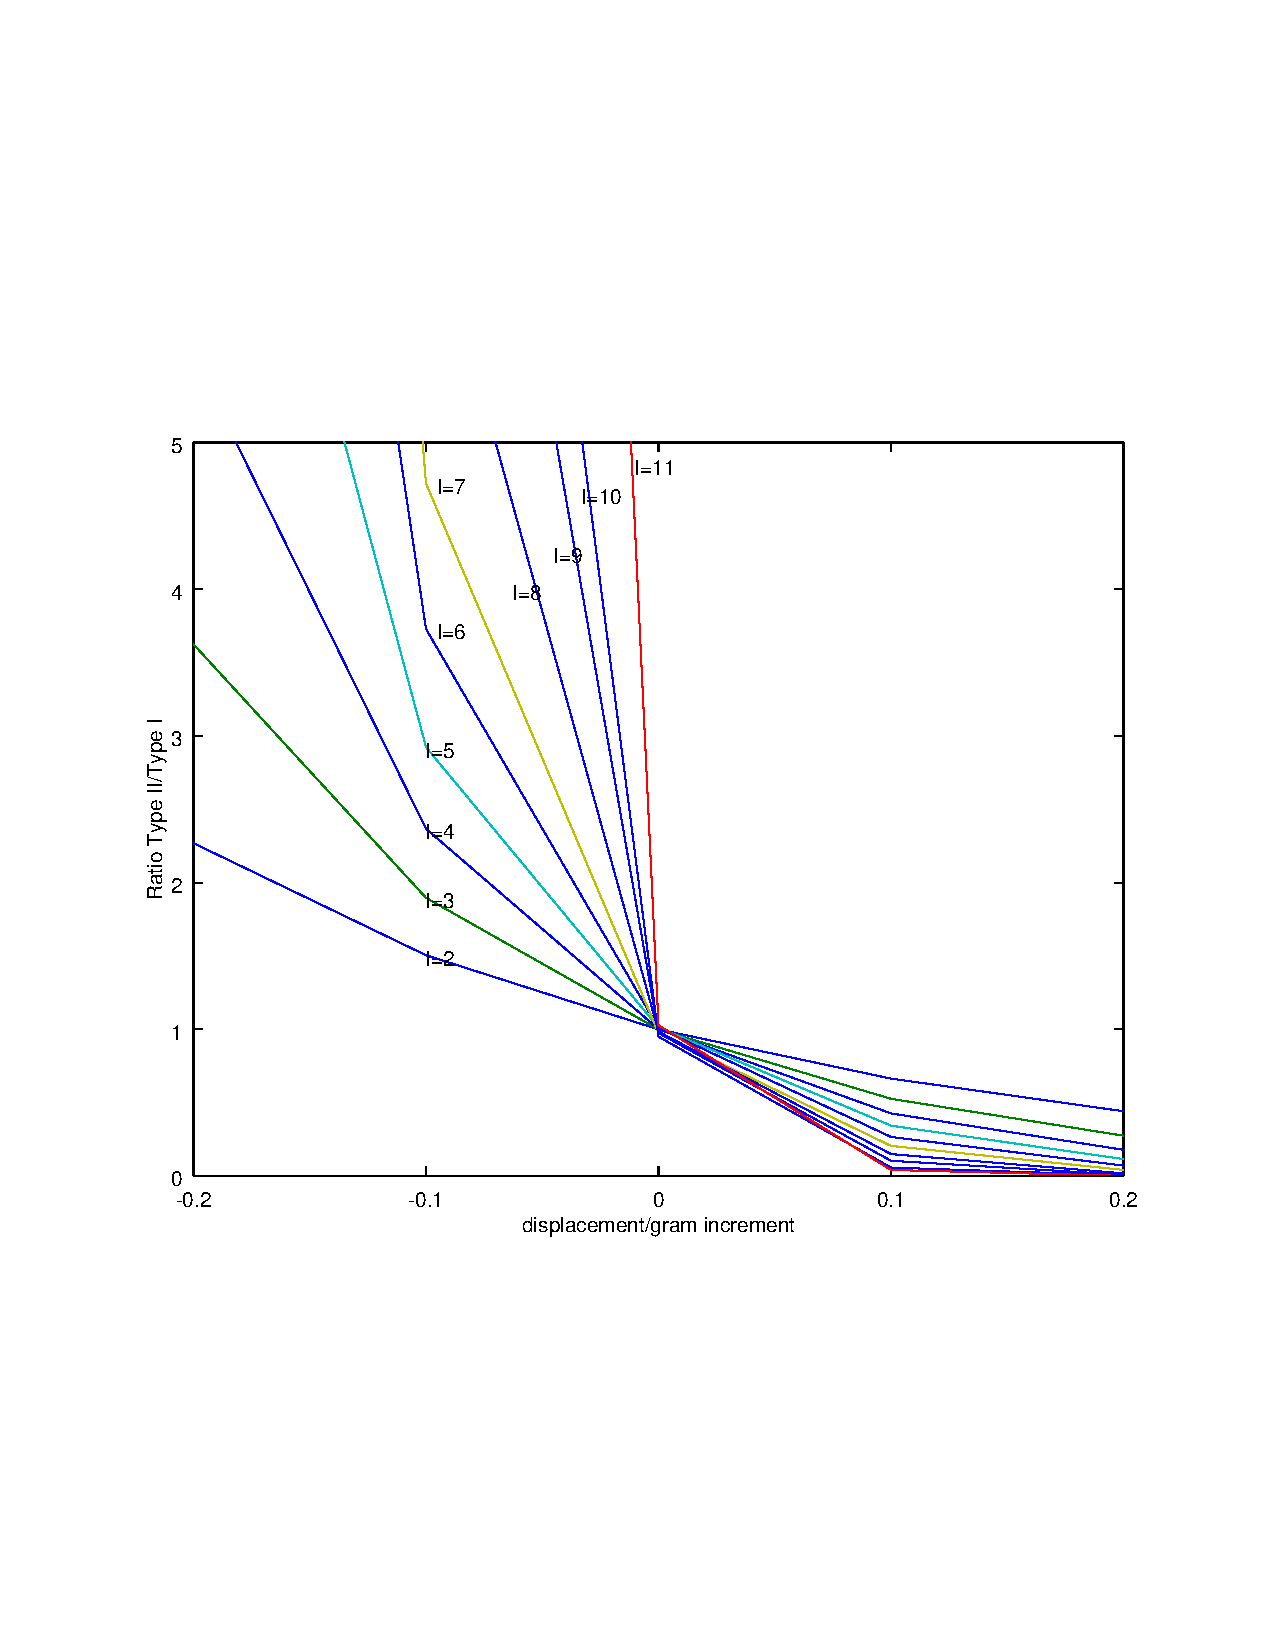
\includegraphics[width=1.1\textwidth]{typeIIratio}
\caption[]{ 
  Ratio of $Type~II/Type~I$ counts for Gram blocks of various lengths $l$, when we displace the Gram points by $n\delta$, where $\delta$ is the Gram interval. All the curves cross over exactly at the Gram point, and have the value $1$ at crossover. Thus, the forward-backward symmetry depends strongly on measuring at the Gram point.
 }
\vspace{1mm}
\label{typeIIratio}
\end{figure}


In this section we investigate further the assumption that that a Gram interval does not differ from any other interval of that length. We study this in the context of the ratio of $Type~II/Type~I$ counts in a given large interval. The starting point is the observation of a remarkable relation, namely, the ratio is very close to one for Gram blocks of different lengths.   Table~\ref{tab:rosser}  (based on data in \cite{gourdon}) shows this fact for all zeros up to $t = 10^{13}$. One question we can ask is the extent to which the results follow just from randomness over and above the basic known patterns of the Riemann zeta distribution. In other words, do the results follow just from the well-known (conjectured) distribution of zero differences on the critical line? Would the results change significantly if we shift all the Gram points  by the same amount in a large interval? We address this question in this section. Table~\ref{tab:rosserrandom} and Figure~\ref{typeIIratio} shows the ratio of $Type~II/Type~I$ counts when we displace the Gram points by $n\delta$, where $\delta$ is the Gram interval. The statistics are from $10$ million Gram intervals at $t=10^{28}$.
They  show clearly that the properties are indeed strongly correlated with the Gram points, and hence are not just manifestations of randomness over and above the basic known patterns of the Riemann zeta distribution. 
We can further study the forward-backward symmetry (and the check that the ratio does depend on whether we measure from Gram points, or from points displaced from Gram points), using the ratio of  $Type~III,left$ interval counts where the '3' interval occurs at the first odd interval position on the left, to  $Type~III,right$ interval counts where the '3' interval occurs at the last odd interval position on the right. 
Table~\ref{tab:rosser3random} shows the ratio of $Type~III,left/Type~III,right$ counts when we displace the Gram points by $n\delta$, where $\delta$ is the Gram interval. This provides further evidence for the conclusions of Table~\ref{tab:rosserrandom}.

  
\begin{table}
\centering \(\begin{array}{cc}
\hline
Type~of~violation &Ratio~of~counts\\
\hline
2L3/2R3 &0.999651352\\
2L22/2R22 &0.999806111\\
3L3/3R3 &0.999217106\\
2L212/2R212 &0.999160495\\
3L22/3R22 &0.999640429\\
4L3/4R3 &0.998017358\\
2L2112/2R2112 &0.998100056\\
2L032/2R230 &0.999734774\\
3L212/3R212 &0.995621266\\
4L22/4R22 &0.998245284\\
2L04/2R40 &0.998111916\\
\hline
\end{array}\)
\caption{Forward-backward symmetry in patterns of violations of Rosser's rule.  The statistics are from the first $10^{13}$ Gram intervals.} \label{tab:vrr}
\end{table}

Further validation comes from a consideration of the different types of violations of Rosser's rule~\cite{gourdon}, which also show the forward-backward symmetry. Rosser's rule states that Gram blocks of length $k$ contain at least $k$ zeros. This law is violated infinitely often, but is violated only for a small fraction of the Gram Blocks. A Gram block is either regular, or it has an excess of zeros, or it has fewer zeros than its length. The last type of Gram block violates Rosser's rule. 
If a Gram block of length k is an exception to Rosser's rule, then its pattern of zeros must be of the form $01...10$. To describe the exception, we must specify where the two missing zeros are. Odlyzko uses the notation $kXa_1a_2 . . . a_m, X = L~or~R $ 
to describe an exception on a Gram block of length $k$  where the missing zeros are on the left (for $X = L$) or on the right (for $X = R$), the pattern containing the missing zeros being $a_1a_2 . . . a_m$ (moreover, this pattern is the smallest union of Gram block adjacent to the exception that contains the missing zeros). For example, $3L04$ denotes a violation of Rosser's rule on a Gram block of length 3, the missing zeros being at its left. Written out in detail, the pattern of zeros is expressed by the notation is $04010$.

The notation above classifies the type of violation of Rosser's rule, the value $m$ being called the length of the excess block. The notation used for exceptions to Rosser's rule is not unambiguous. When several contiguous violations of Rosser's rule exists, they may overlap or missing zeros can be in the same Gram interval. Such situations are very rare, and in these cases (Gourdon found just three occurrences until the $10^{13}th$ zero), Odlyzko uses the notation $Ma_1 ...a_l$ where the pattern $a_1 . . . a_l$ is made of the minimal contiguous Gram blocks containing at least one violation to Rosser rule, and all the missing zeros. For example, the pattern $M00500$, first encountered at gram index $n = 3,680,295,786,518$, denotes a situation with two violations of Rosser's rule ($00$ and $00$, Gram blocks with missing zeros) and a single Gram interval containing all the missing zeros (pattern $5$). 
Table~\ref{tab:vrr}  (based on data in \cite{gourdon}) shows the forward-backward symmetry in patterns of violations of Rosser's rule. Once again, while there is very good evidence for the forward-backward symmetry, the $L$ type violations are ever so slightly smaller than the $R$ type violations. Again, we have evidence for a symmetry which is broken very slightly.

In the next section we present two new conjectures based on the empirical evidence presented so far.


\section{\label{sec7}Two Conjectures}

\begin{figure*}
\centering
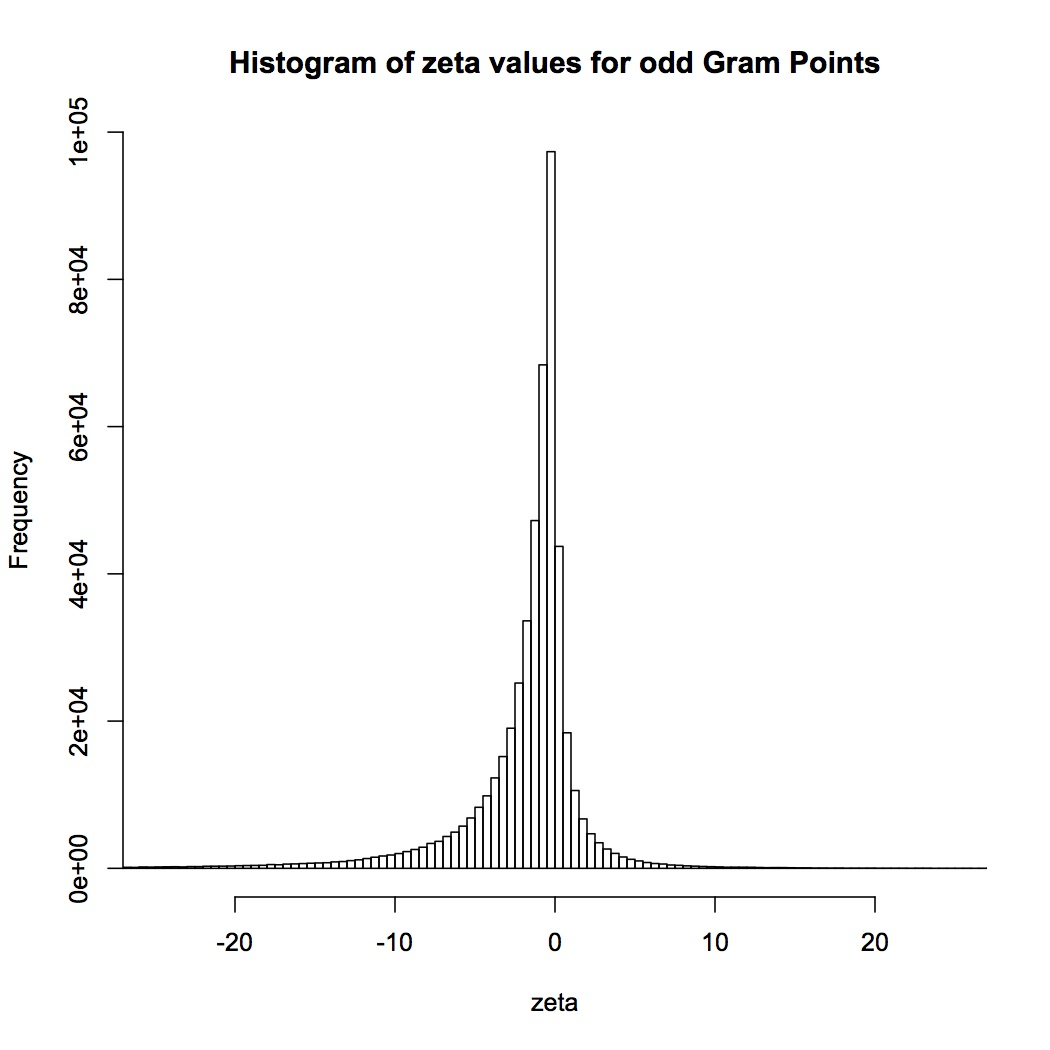
\includegraphics[width=0.62\textwidth]{ozeta.jpg}
\caption[]{ 
  Distribution of zeta values at 500000 odd Gram points  at $t = 10^{12}$.
 }
\vspace{1mm}
\label{oddhist}

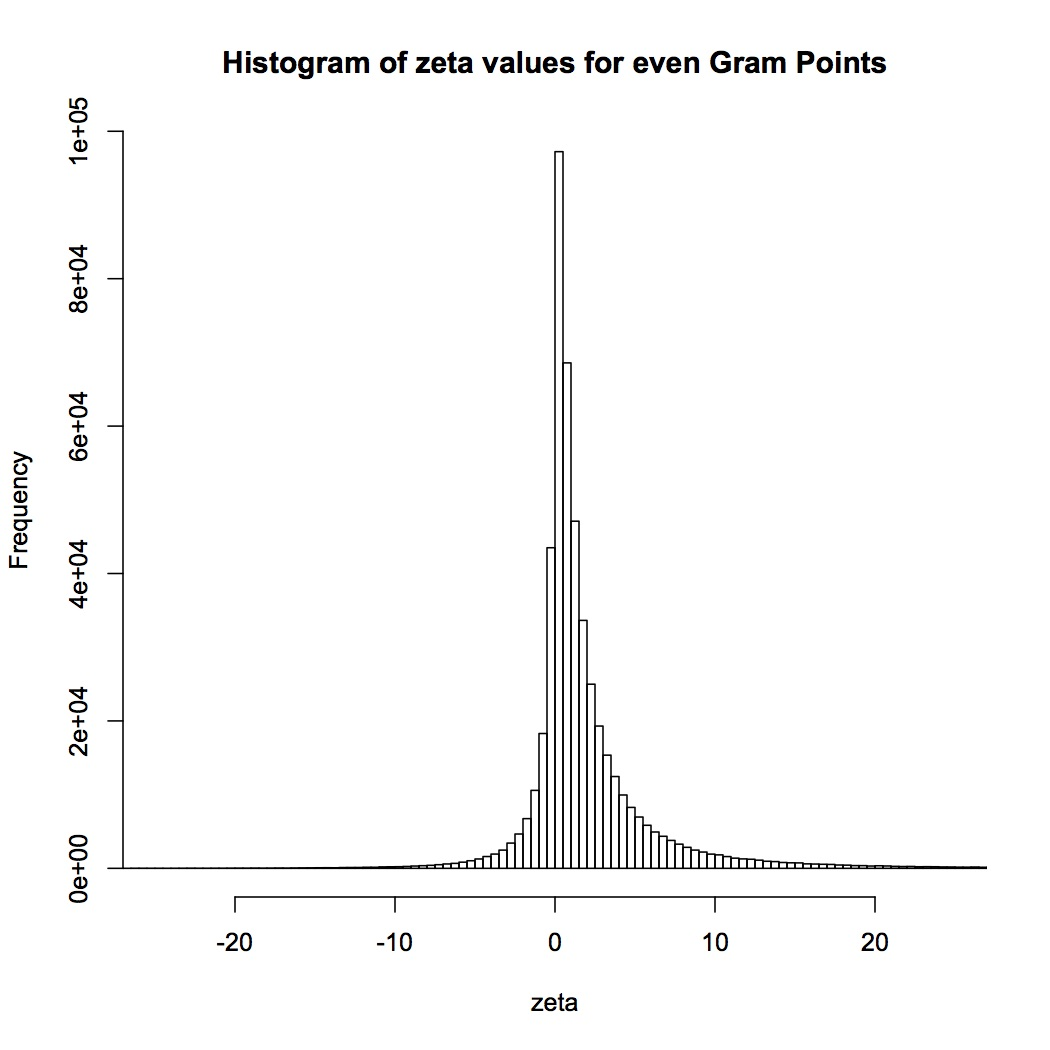
\includegraphics[width=0.62\textwidth]{ezeta.jpg}
\caption[]{ 
   Distribution of zeta values at 500000 even Gram points  at $t = 10^{12}$.
 }
\label{evenhist}
\vspace{1mm}
\end{figure*}

\begin{table}
\centering \(\begin{array}{ccccccc}
\hline
 Gram &     Min.   & 1st    &  Median    &   Mean   & 3rd    &   Max. \\
 type &              & Quantile   &            &              & Quantile.    &   \\
\hline
All& -160.90 &   -1.17 &    0.00106 &   0.00  &  1.172 &165.10\\
Odd&-160.90 &   -2.526 &   -0.8471  & -2.00 &   -0.1121 &  69.41 \\
Even&-68.63 &   0.1139 &  0.8526  & 2.00 &   2.541 & 165.10 \\
\hline
\end{array}\)
\caption{Quantiles and mean for zeta values at Gram points of different types.  The statistics are from $1$ million Gram intervals at $t=10^{12}$.} \label{tab:quantiles}
\end{table}


\begin{table}
\centering \(\begin{array}{ccccc}
\hline
 Gram~type&   --   & -+   & +-   & ++  \\
\hline
Odd & 0.151651&0.627465&0.069119&0.151765 \\
Even & 0.151565&0.069206&0.627551&0.151678 \\
\hline
\end{array}\)
\caption{Counts of different configurations of zeta values for pairs of consecutive Gram points.  The statistics are from $10$ million Gram intervals at $t=10^{15}$.} \label{tab:pairraw}
\end{table}

\begin{table}
\centering \(\begin{array}{ccccc}
\hline
 Gram~type&   --   & -+   & +-   & ++  \\
\hline
Odd & 0.151651&0.627465&0.069119&0.151765\\
\hline
Corresponding& 0.151678 & 0.627551 & 0.069206& 0.151565\\ 
Even~Entry     & (++)     & (+-)   & (-+)  & (--) \\
\hline
\end{array}\)
\caption{Test of Conjecture \ref{antisymmetry} using pairs of consecutive Gram points.  The statistics are from $10$ million Gram intervals at $t=10^{15}$.} \label{tab:pairtest}
\end{table}


The empirical data presented in the previous section lead us to formulate two new conjectures  about the distribution of zeta values at the 
the Gram points. These conjectures are most likely related to the symmetry properties of the rotated zeta function (Hardy's function) under inversion around the origin. 

\begin{mydef}\label{antisymmetry}
(even-odd antisymmetry): The distribution of the zeta values for odd Gram points is the negative of the distribution of zeta values for the even Gram points.
\end{mydef}
\begin{mydef}\label{symmetry}
(forward-backward symmetry): When we consider a sequence of zeta values at consecutive Gram points, the properties of the sequence are symmetric with respect to the direction of the sequence of Gram points (i.e., the sequence behaves similarly whether we consider the points in increasing order or in decreasing order).
\end{mydef}

The evidence for  Conjecture~\ref{symmetry} has been presented in the previous sections. 
In this section we will consider the statistics of zeta values at pairs of consecutive Gram points. We will look at the evidence for Conjecture \ref{antisymmetry}.  All the data  are from $10$ million Gram intervals starting at $t=10^{15}$.

Figures \ref{oddhist} and ~\ref{evenhist}  present the histograms of zeta values at odd Gram points and even Gram points respectively. These figures further bear out the evidence of Table~\ref{tab:quantiles} that the odd and even distributions are mirror images of each other. To study Conjecture \ref{antisymmetry} further, we will consider the zeta values at pairs of consecutive Gram points. We will classify the zeta values into two classes, '$+$' for positive zeta values ($zeta > 0$) and '$-$' for negative zeta values ($zeta \leqslant  0$). Thus, for example, the notation '$++$' stands for a Gram Point which has a positive zeta value followed by a Gram Point which has a positive zeta value, while the notation '$+-$' stands for a Gram Point which has a positive zeta value followed by a Gram Point which has a negative zeta value. Table~\ref{tab:pairraw} shows the counts for different pair configurations, for pairs beginning at odd Gram points (row 1) and for pairs beginning at even Gram points(row 2). Conjecture \ref{antisymmetry} predicts that the count for a configuration from the odd Gram point row in the table  will match the count for the mirror configuration in the even Gram point row of the table ( e.g., the count for '$++$' from the distribution for odd Gram points will match count for '$--$' from the distribution for even Gram points). Table~\ref{tab:pairtest} tests this prediction. The agreement is good, within the expected statistical variations. 

In the next section we present the conclusions.


\section{\label{conclusions}Conclusions}

In this work we presented a new  relation for the ratio of good to bad Gram points. We presented two conjectures regarding the distribution of zeta function values at Gram points. The conjectures refer to the even-odd Gram point antisymmetry and the forward-backward symmetry ("time reversal" symmetry, if we think of the zeta values at Gram points as being a time series). After briefly describing the theory of the Riemann zeta function and the numerical evaluation, we presented statistics of the zeta function values. The statistics provide validation for the two conjectures.


\begin{thebibliography} {}

\bibitem{Sarnak 2005} Peter Sarnak,
"Problems of the Millennium: The Riemann Hypothesis (2004)", The Proceedings of the Clay Mathematics Institute 2004, Budapest, Hungary,
\url{http://www.claymath.org/sites/default/files/sarnak_rh_0.pdf}, (2005)

\bibitem{Gram 1903} J. P. Gram, 
"Sur les Zeros de la Fonction  $\zeta ( s )$  de Riemann",
{\it Acta Math.} {\bf27}(1903), 289-304.

\bibitem{Odlyzko 1992}  A. Odlyzko,
"The $10^{20}$-th Zero of the Riemann Zeta
Function and 175 Million of its Neighbors'", report,
\url{http://www.dtc.umn.edu/~odlyzko/unpublished/zeta.10to20.1992.pdf}, (1992)


\bibitem {Riemann(1858)} B. Riemann, ``\"{U}ber die Anzahl der Primzahlen uter
Einer Gegebenen Gr\"{o}be,'' {\it Montasb. der Berliner Akad.}, (1858),
671-680.

\bibitem {Riemann 1892} B. Riemann, ``Gesammelte Werke'', Teubner, Leipzig, (1892).

\bibitem {Titchmarsh 1986} E. Titchmarsh, ``The Theory of the Riemann Zeta
Function,'' Oxford University Press, Second Edition, (1986).

\bibitem {Edwards(1974)} H. M. Edwards, ``Riemann's Zeta Function,'' 
Academic Press,  (1974).

\bibitem{os6} O. Shanker, 
"Generalised Zeta Functions and Self-Similarity of Zero Distributions",
{\it J.  Phys. A} {\bf39}(2006), 13983-13997.

\bibitem {Matiyasevich} Y. Matiyasevich, 
"An artless method for calculating approximate values of
zeros of Riemann zeta function",
Web report, \url{http://logic.pdmi.ras.ru/~yumat/
personaljournal/artlessmethod/artlessmethodtexts.php}, (2013)

\bibitem{hiary} G. A. Hiary,
"METHODS TO COMPUTE THE RIEMANN ZETA
FUNCTION", arxiv.org, math.NT, 0711.5005v4, (2011).

\bibitem{gourdon} Xavier Gourdon,
"The $10^{13}$ first zeros of the Riemann Zeta function,
and zeros computation at very large height", report,
\url{http://numbers.computation.free.fr/Constants/Miscellaneous/zetazeros1e13-1e24.pdf}, (2004)

\bibitem {Odlyzko(1989)} A. Odlyzko, "The $10^{20}$-th Zero of the Riemann Zeta
Function and 70 Million of its Neighbors'' (preprint), A.T.T., (1989).


\end{thebibliography} 

\end{document} 
